\documentclass[a4paper,10pt,notitlepage]{scrreprt}

\usepackage[T1]{fontenc}
\usepackage[english]{babel}
\usepackage[utf8x]{inputenc}
\usepackage{setspace}
\usepackage{subfig}
\usepackage{textcomp}
\usepackage{graphicx}
\usepackage{fixltx2e}
\usepackage{multirow}
\usepackage{array}
\usepackage{amssymb}
\usepackage{amsmath}
\usepackage{subfig}
\usepackage{nomencl}
\usepackage[pdfborder={0 0 0}]{hyperref}
\usepackage{natbib}
% \usepackage{makeidx}
\usepackage{nicefrac}
\usepackage{bbold}

\captionsetup{labelfont=footnotesize,textfont=footnotesize}

\newcolumntype{x}[1]{>{\begin{flushleft}$}p{#1}<{$\end{flushleft}}}
\newcolumntype{y}[1]{>{\begin{center}$}p{#1}<{$\end{center}}}
\newcolumntype{z}[1]{>{\begin{flushright}$}p{#1}<{$\end{flushright}}}
\newcolumntype{m}{>{$}l<{$}}
\newcolumntype{n}{>{$}c<{$}}
\newcolumntype{o}{>{$}r<{$}}

\bibliographystyle{plain}

% Title Page
\title{Scientific Visualization\\Project II}
\author{Milian Wolff}


\begin{document}
\maketitle

\begin{abstract}
Our second project in the scientific visualization class by Eugene Zhang gave
us the opportunity to get acquainted with the algorithms behind ``pen-and-ink
sketching'' of a 3D mesh surface. First we explore the steps required to
visualize silhouettes of a geometry. Then we calculate the vertex-based
curvature and curvature tensors. Finally we will combine the both to draw a
sketch-like version of a given geometry.

The source code of my exercise solutions can be found online under

\begin{center}\url{https://github.com/milianw/scivi}\end{center}
\end{abstract}

\begingroup
\let\clearpage\relax

\tableofcontents
\endgroup

\chapter{Corner Table}

As a foundation for the later tasks we first had to implement a corner table. I
did this by following the steps outlined in class:

\begin{itemize}
 \item iterate over all triangles
 \item add each corner in the triangle to a table
 \item sort table by $min(c.prev.vertex, c.next.vertex)$ and
$max(c.prev.vertex, c.next.vertex)$
 \item iterate over sorted table and associate consecutive rows with equal
$min$ and $max$ entries as opposite corners
\end{itemize}

The implementation can be found in \texttt{CornerTable.java}.

The resulting corner table is essentially a linked list which is straight
forward to use. I additionally added a \texttt{Corner[] vertexNeighbors()}
method to my \texttt{Corner} object, which essentially returns the $N^1$-ring
vertex neighbors.

\section{Validation}

To verify the correctness of my implementation of a corner table, I wrote
\texttt{Ex2\_1.java}. When started, the user defines a geometry. Then the corner
table for said geometry is computed. Now we iterate over each corner \texttt{c}
and run a set of assertion-based tests in each step:

\begin{itemize}
 \item \texttt{c.next != null}
 \item \texttt{c.prev != null}
 \item \texttt{c.next.triangle != c.triangle}
 \item \texttt{c.prev.triangle != c.triangle}
\end{itemize}

Furthermore, the correctness of the ``opposite''-association is validated by
asserting the following tests:

\begin{itemize}
 \item \texttt{c.triangle != c.opposite.triangle}
 \item \texttt{c.next.vertex == c.opposite.prev.vertex}
 \item \texttt{c.prev.vertex == c.opposite.next.vertex}
 \item \texttt{c == c.opposite.opposite}
 \item \texttt{c.prev.opposite.next.vertex == c.next.vertex}
 \item \texttt{c.prev.opposite != c.next}
 \item \texttt{c.prev.opposite.prev.vertex == c.vertex}
 \item \texttt{c.prev.opposite.prev != c}
 \item \texttt{c.next.opposite.prev.vertex == c.prev.vertex}
 \item \texttt{c.next.opposite.prev != c.prev}
 \item \texttt{c.next.opposite.next.vertex == c.vertex}
 \item \texttt{c.next.opposite.next != c}
\end{itemize}

Keep in mind though that in open surfaces like e.g. \texttt{Gauss\_3042.byu} not
every corner can be associated to an opposite one. This is handled gracefully in
my corner table implementation and unit tests.

Another implicit verification of my implication lies in the extensive usage of
the corner table in the following exercises. Since the solutions there seem to
be visually correct, the corner table seems to yield correct results.

\chapter{Silhouette}

Now we want to find the silhouette of a 3D geometry using two different
algorithsm. My solutions to both can be found in \texttt{Silhouette.java} and
\texttt{Ex2\_2.java}.

\section{Face-based approach}

The first task was to find the silhouette by iterating over all edges and
finding those, where only one of the adjacent triangles is ``visible''. Here, we
consider a triangle $T$ to be visible when

\begin{equation}
 (\vec{c}_T - \vec{v}) \cdot \vec{n}_T < 0,
\end{equation}

with $\vec{c}_T$ being the center and $\vec{n}_T$ being the normal of the
triangle respectively. $\vec{v}$ is the position of the viewer.

Note that this approach yields undefined results for triangles that are
exactly perpendicular to the view ray. There, the dot product will be zero and
the triangle is either an invisible backside or a visible frontside. I ignore
these edges, assuming that this case only happens for faces somewhere in the
middle of the (in-)visible surface and are thus not part of the silhouette
anyways.

Now to actually find the silhouette, I first iterate over all triangles and
store the associated index to a list $L$ when the triangle is visible. Then
I iterate over the corner table and find corners $c$ within a visible triangle,
i.e. $c.triangle$ is contained in $L$. Then the edge between $c.prev.vertex$
and $c.next.vertex$ is part of the silhouette, if either $c.opposite$ is
undefined, or alternatively $c.opposite.triangle$ is not contained in $L$.

My implementation of the above can be found in
\texttt{Silhouette.createFaceBasedSilhouette()}.

\subsection{Problems}

The silhouette is view dependendend and \texttt{Ex2\_2} hence recalculates the
silhouette whenever the view point changes. Now when rotating a given geometry,
the main problem of this approach becomes apparent: Gradual changes in the view
can have a big difference one the silhouette. Comparing e.g. fig.
\ref{fig:face-silhouette-bunny-1} and \ref{fig:face-silhouette-bunny-2} shows
this issue at the right ear. Additionally we also see three artifacts, two on
the body and one at the left eye.

The same issue is also responsible for the jagged edge of the sphere silhouette
as visible in fig. \ref{fig:face-silhouette-sphere}. 

\begin{figure}
  \subfloat[]{
    \label{fig:face-silhouette-bunny-1}
    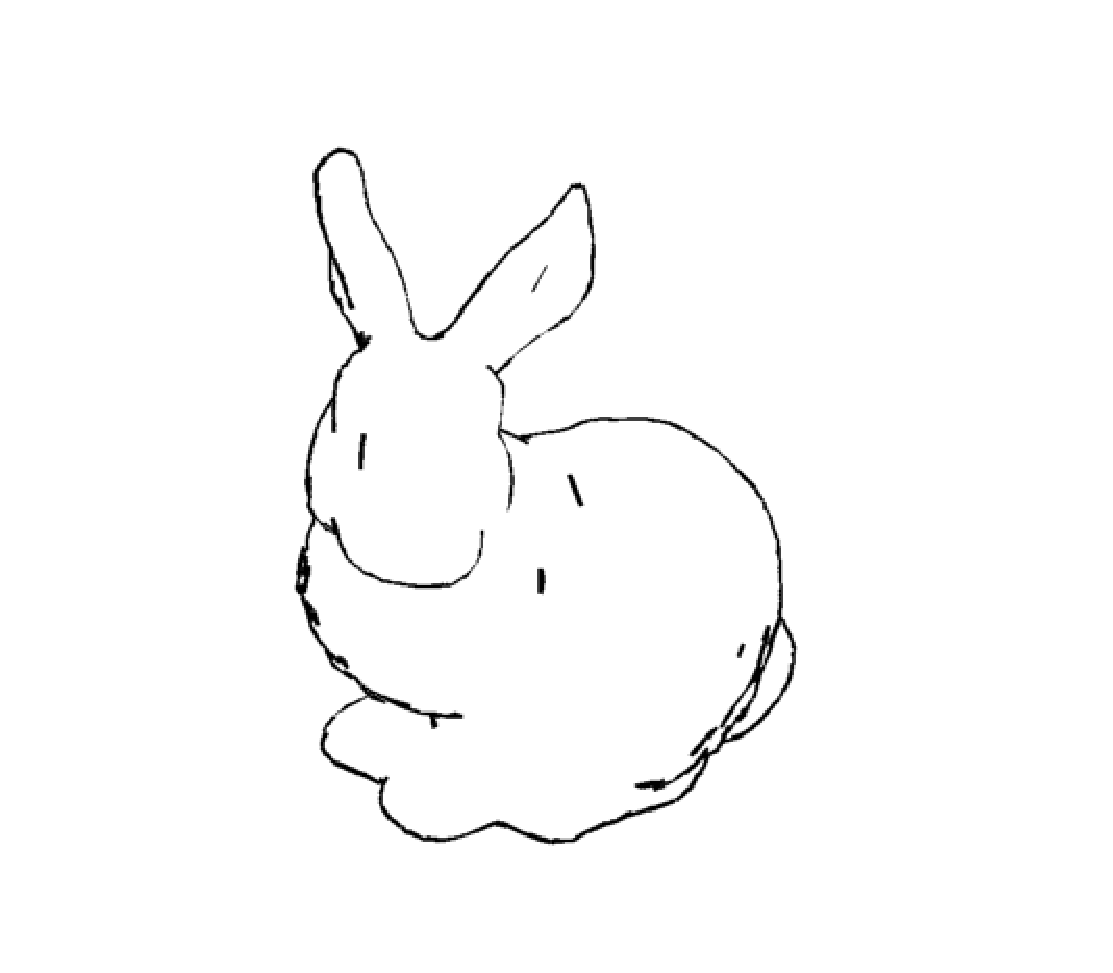
\includegraphics[scale=0.4]{img-2-2/bunny-1.eps}}
  \subfloat[]{
    \label{fig:face-silhouette-bunny-2}
    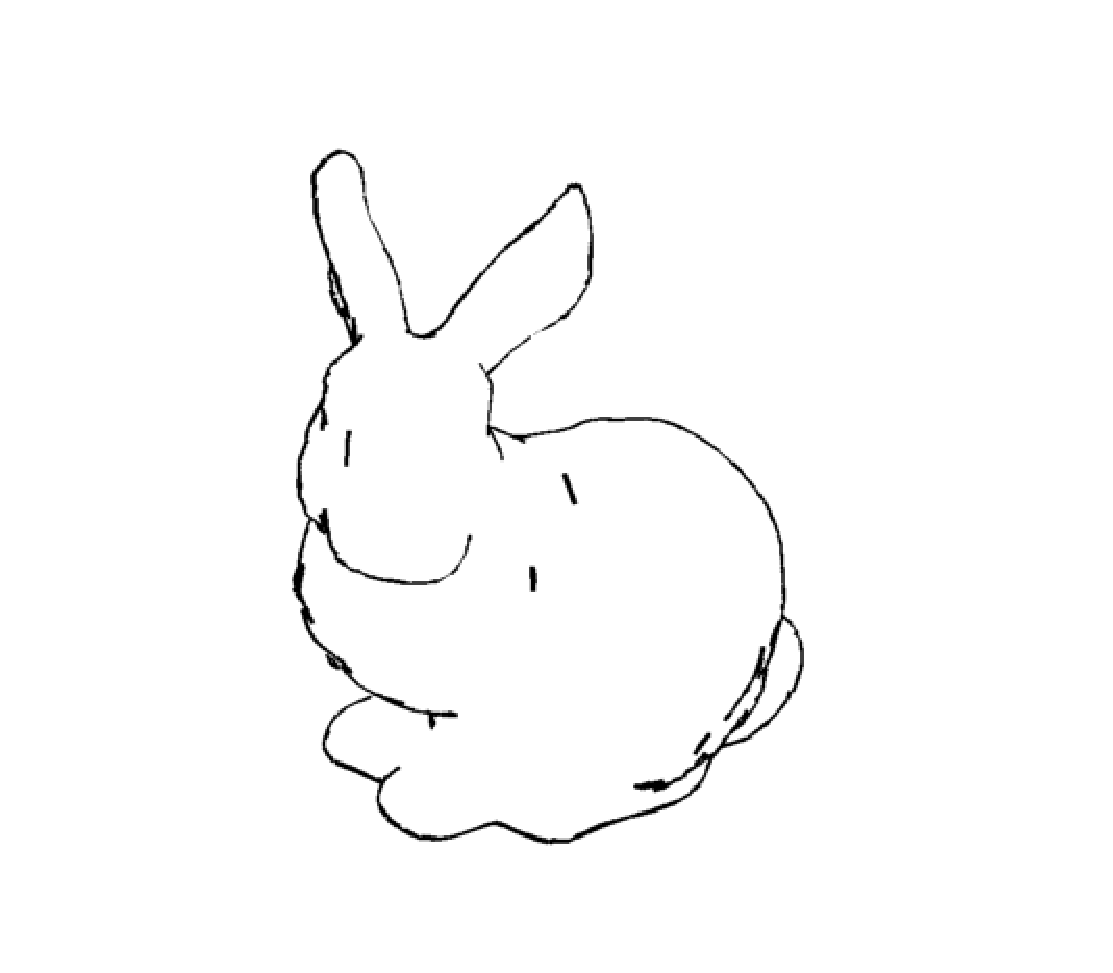
\includegraphics[scale=0.4]{img-2-2/bunny-2.eps}}
 \caption{Face-based silhouette of the bunny under slight rotation}
 \label{fig:face-silhouette-bunny}
\end{figure}

\section{Vertex-based approach / zero level set}

In an attempt to fix the issues of our first approach, we now apply a different
scheme that computes the so called zero level set. That is the curve on the
surface where the dot product between the curve normal and the view ray is
always zero.

To compute this curve we iterate over the corner table and calculate the dot
product between the view ray and the normal at the corner vertex $c$ and its
previous and next vertex $p$ and $n$:

\begin{eqnarray}
 d_{c} = a = (\vec{c} - \vec{v}) \cdot \vec{n}_c \\
 d_{p} = b = (\vec{p} - \vec{v}) \cdot \vec{n}_p \\
 d_{n} = c = (\vec{n} - \vec{v}) \cdot \vec{n}_n
\end{eqnarray}

If we then encounter a triangle where either $a \leq 0$, $b \geq 0$ and $c \geq
0$ or $a \geq 0$, $b \leq 0$ and $c \leq 0$, then a zero level set line goes
through this triangle. We assume it can be approximated
linearly interpolating $a$ and $b$ onto the edge between $c$ and $p$ and
analogously for $a$ and $c$ and then connecting the two points for which the
interpolated dot product should yield zero.

The code for my implementation can be found in
\texttt{Silhouette.createVertexBasedSilhouette()} and
\texttt{Silhouette.findZeroLevel()}.

\subsection{Comparison}

The vertex-based silhouette yields mostly better results, as can be seen in
e.g. figs. \ref{fig:silhouette-sphere} or \ref{fig:silhouette-dragon}.

Interestingly enough though, the face-based approach seems to yield a more
detailed silhouette for the feline, see fig. \ref{fig:face-silhouette-feline}.
Since we are looking for the actual silhouette though, the face-based approach
seems to be more correct though.

\begin{figure}
  \subfloat[face-based]{
    \label{fig:face-silhouette-sphere}
    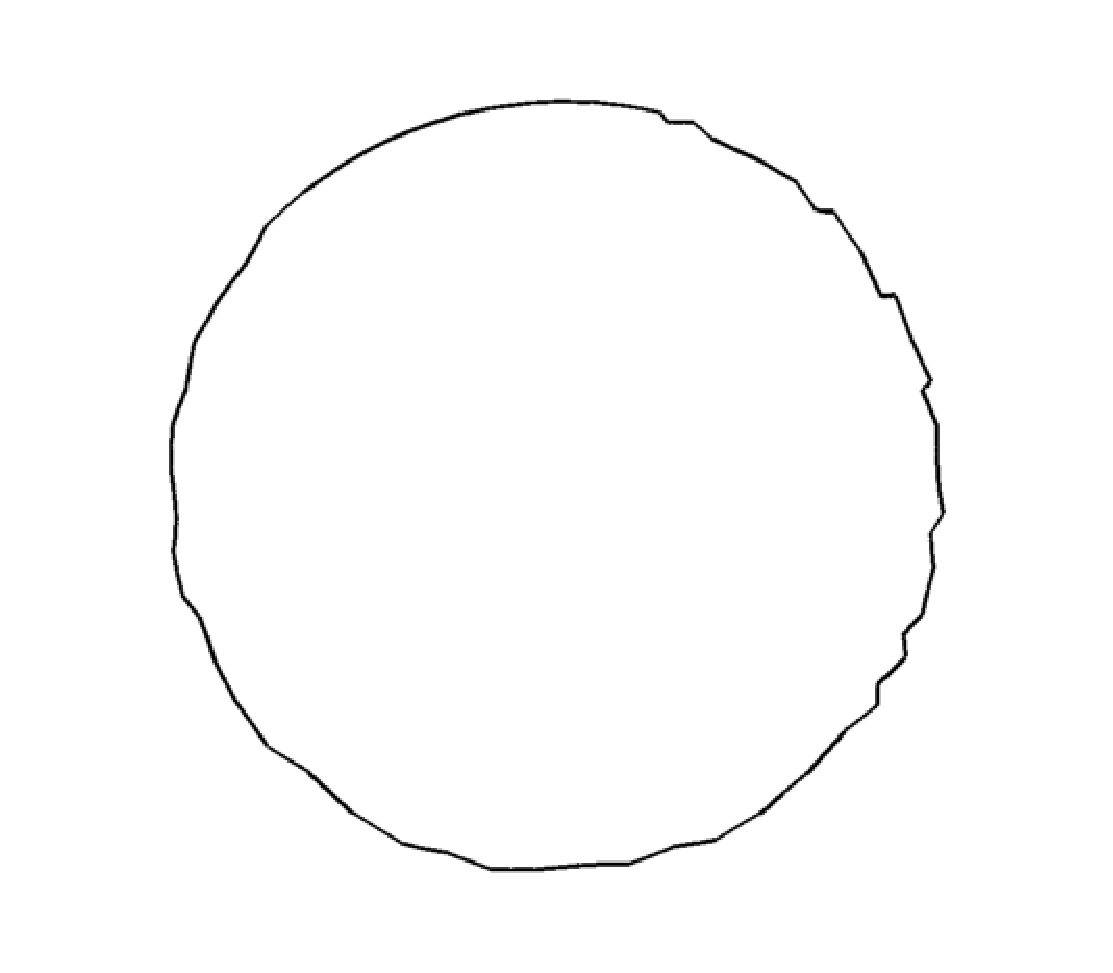
\includegraphics[scale=0.4]{img-2-2/sphere-face.eps}}
  \subfloat[vertex-based]{
    \label{fig:vertex-silhouette-sphere}
    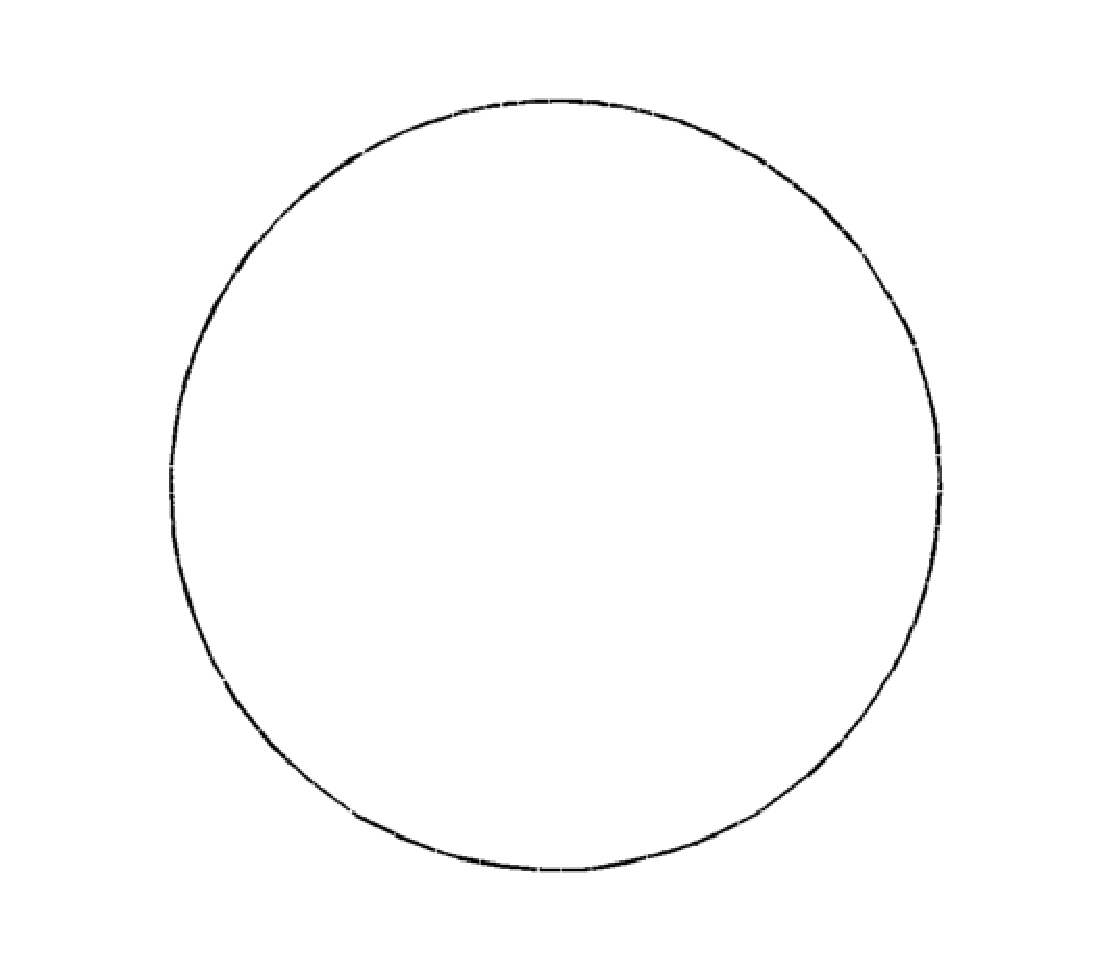
\includegraphics[scale=0.4]{img-2-2/sphere-vertex.eps}}
 \caption{Comparison of face- and vertex-based silhouette for the sphere}
 \label{fig:silhouette-sphere}
\end{figure}

\begin{figure}
  \subfloat[face-based]{
    \label{fig:face-silhouette-dragon}
    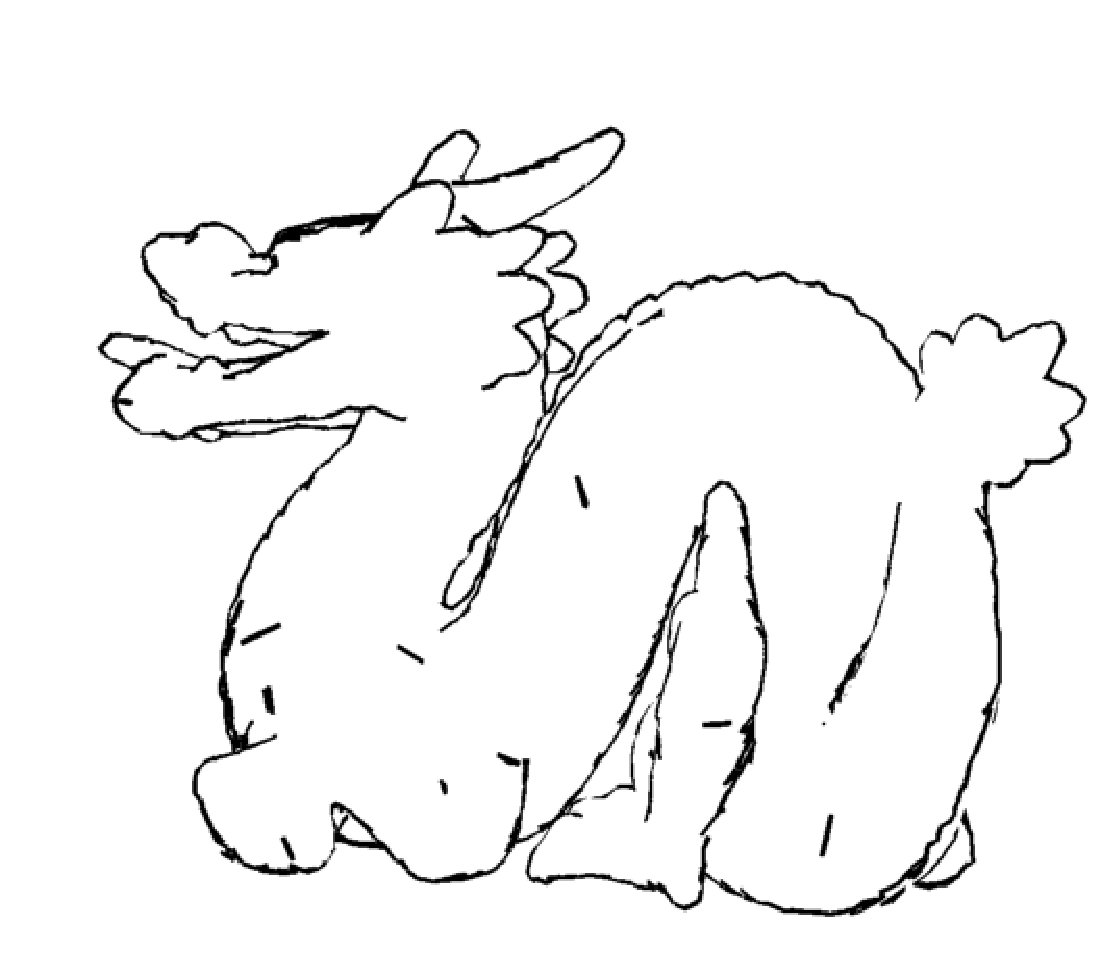
\includegraphics[scale=0.4]{img-2-2/dragon-face.eps}}
  \subfloat[vertex-based]{
    \label{fig:vertex-silhouette-dragon}
    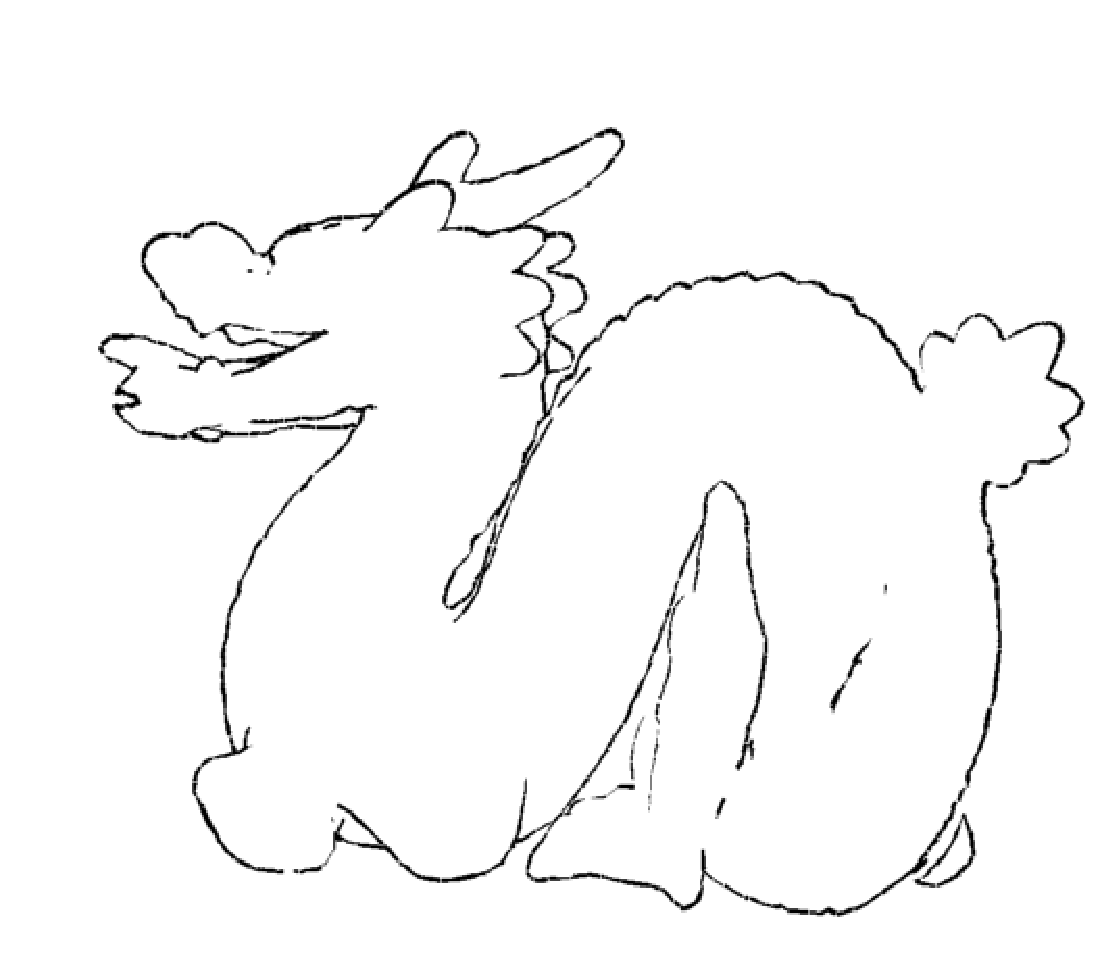
\includegraphics[scale=0.4]{img-2-2/dragon-vertex.eps}}
 \caption{Comparison of face- and vertex-based silhouette for the dragon}
 \label{fig:silhouette-dragon}
\end{figure}

\begin{figure}
  \subfloat[face-based]{
    \label{fig:face-silhouette-feline}
    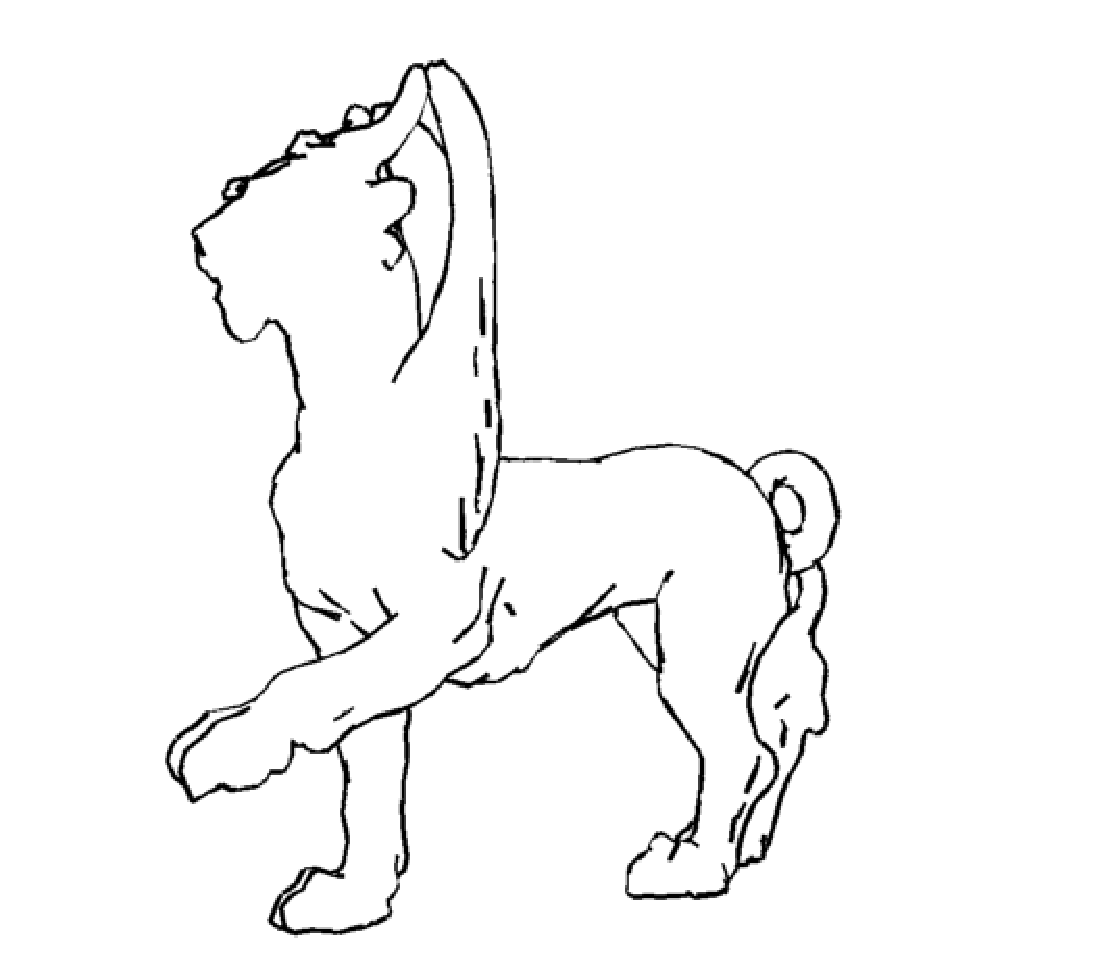
\includegraphics[scale=0.4]{img-2-2/feline-face.eps}}
  \subfloat[vertex-based]{
    \label{fig:vertex-silhouette-feline}
    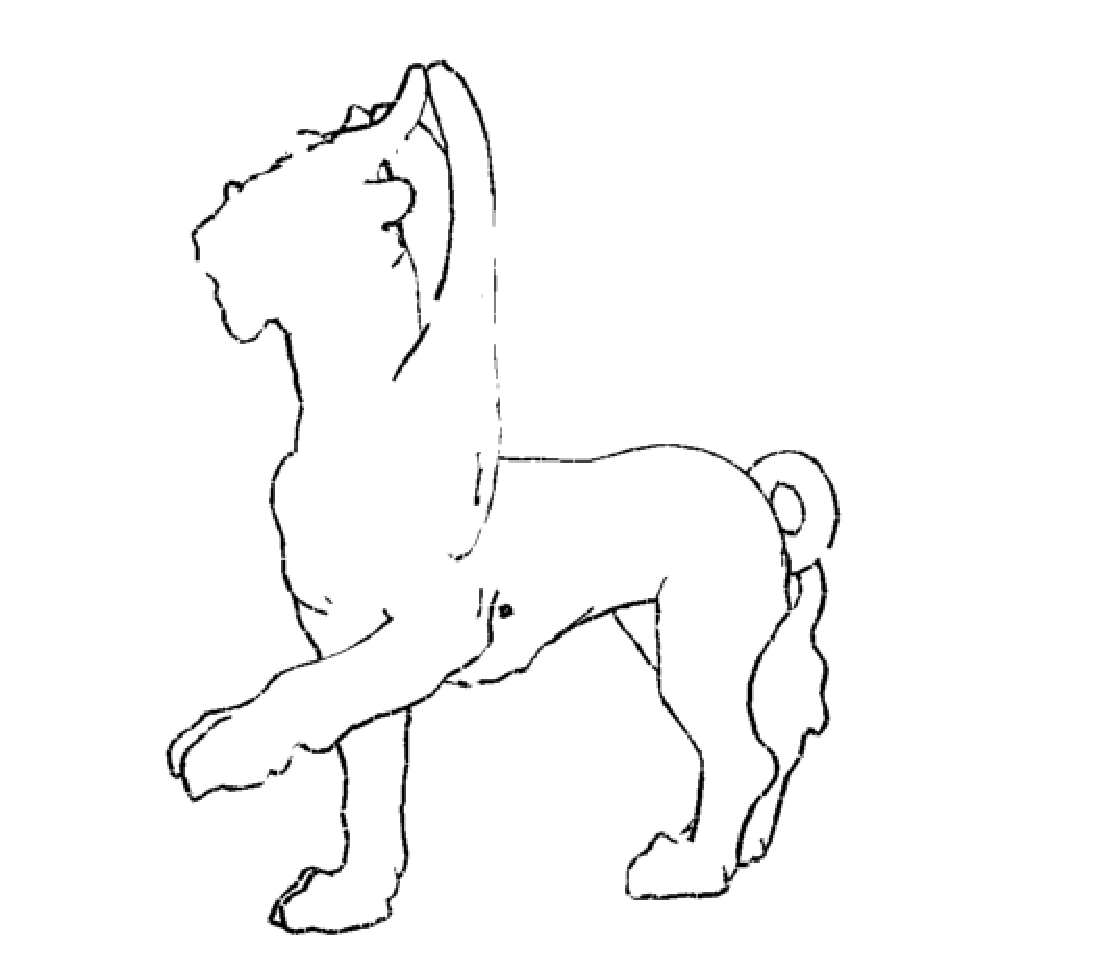
\includegraphics[scale=0.4]{img-2-2/feline-vertex.eps}}
 \caption{Comparison of face- and vertex-based silhouette for the feline}
 \label{fig:silhouette-feline}
\end{figure}

\section{Silhouette in JavaView}

To actually draw the silhouette in JavaView, one has to add the edges to a
\texttt{PgPolygonSet} using \texttt{addPolygon()}. Furthermore we must prevent
painting of obscured parts of the silhouette, which can be achieved by
keeping the original geometry in the display but coloring its elements
completely white using \texttt{PgElementSet.setGlobalElementColor(Color.white)}
and by disabling lightning via
\texttt{PvDisplayIf.setLightingModel(PvLightIf.MODEL\_SURFACE)}.

\chapter{Curvature estimation}

TODO: paper source



% \bibliography{sources}

\end{document}

% kate: replace-tabs on;